\documentclass[12pt]{scrartcl}
\usepackage{authblk}
\usepackage{amsmath}
\usepackage{FiraSans}
\usepackage{siunitx}
\usepackage{natbib}
\usepackage[dvipsnames]{xcolor}
\usepackage[pdftex,
bookmarksnumbered=true,
colorlinks=true,
linkcolor=Blue,
citecolor=Gray,
urlcolor=ForestGreen,
pdfpagelabels=false,
plainpages = false,
]{hyperref}
\usepackage[capitalise]{cleveref}
\usepackage{graphicx}
\graphicspath{
{./figures/}}
\DeclareGraphicsExtensions{.pdf,.png,.gif}


\newcommand{\myscale}{1}

\begin{document}

\title{
Tomography characterization of solid oxide fuel cells using high-energy transmission x-ray microscopy}
\author[a]{Chen Zhang}
\author[b]{P. Kenesei}
\author[b]{S. D. Shastri}
\author[a]{R. M. Suter}

\affil[a]{Department of Physics, Carnegie Mellon University, Pittsburgh, PA, USA}
\affil[b]{Advanced Photon Source, Argonne National Laboratory, Argonne, IL, USA}

\maketitle

% ----- Motivation ----- %
\section{Motivation}\label{sec: motivation}

High-energy transmission x-ray microscopy (HETXM) can provide tomography characterization with sub-micron spatial resolution for samples that are too thick for conventional nano-CT characterization \citep{Shastri_etal2015}.
In this study, the tip region ($20\times20\times\SI{100}{\micro\meter}$) of a solid oxide fuel cell (SOFC) was characterized using HETXM.
The sinograms collected from the HETXM experiment were used to reconstruct the morphology of the tip using open source tomography reconstruction suite TomoPy \citep{Gursoy_etal2014}, the results of which were used to evaluate the porosity state of the tip of the SOFC. 


% ----- Experiment ----- %
\section{Experiment}\label{sec: exp}

The HETXM experiment was performed at the advanced photon source beamline 1-ID in the Argonne national laboratory using the standard HETXM configuration developed by \citet{Shastri_etal2015}.
A total number of six tomography scans were conducted at \SI{\sim 50}{keV} using a far-field detector ($2048\times2048$ pixel resolution) with a step size of \ang{0.1}, resulting in an effective detection resolution of $\SI{200}{nm/pixel}$.
Although all six tomography scans covering different regions of the SOFC pillar yielded projection images suitable for tomography reconstruction, only the tip of the SOFC was reconstructed and analyzed in this study, mostly as a proof of concept.


% ----- Tomo recon ----- %
\section{Tomography reconstruction}\label{sec: tomo}

\subsection{Data preprocessing}\label{sec: preprocessing}

The reflective lenses and the associated sub-micron resolution of HETXM makes the collected projection images more sensitive to the beam instability (beam wiggling and intensity fluctuation) and dynamic misalignment \footnote{
The far-field detector can tilt and drift slightly with respect to the beam axis during the experiment, and the associated artifacts can be amplified by the HETXM configuration.
} 
when compared with conventional high-energy tomography characterization.
Therefore, projection images collected from HETXM need to be corrected for both factors prior to tomography reconstruction.

\subsubsection{
Correction for beam instability
}\label{sec: bg norm}

Similar to conventional tomography characterization, the projection images collected from HETXM contains beam characteristics, which can be in theory removed by subtracting the flat field images (\cref{fig: flat field images}) following Beer's law. 
However, the beam wiggling (spatial instability) and beam intensity fluctuation (temporal instability) can leave residual beam characteristics in the normalized projection images.
Consequently, advanced background normalization is necessary to further minimize these residual beam characteristics.

% --- background images --- %
\renewcommand{\myscale}{0.4}
\begin{figure}[htp]
\centering
\small
\begin{tabular}{cccc}
	 White field (before)
&  White field (after)
&  White field difference
&  Dark field (after)
\\
  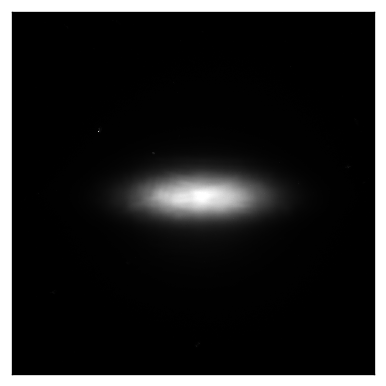
\includegraphics[scale=\myscale]{whiteField_pre}
& 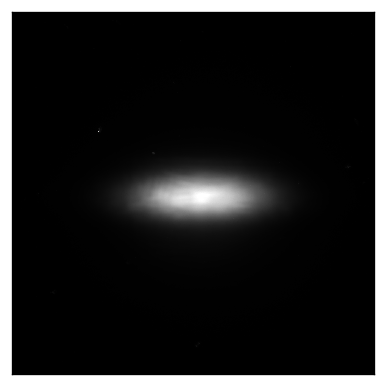
\includegraphics[scale=\myscale]{whiteField_pst}
& 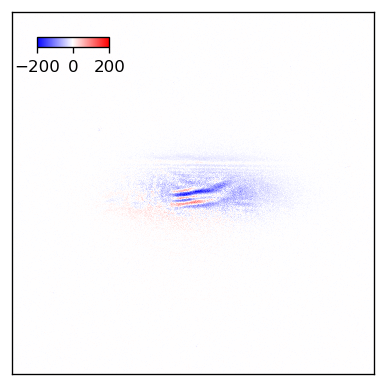
\includegraphics[scale=\myscale]{whiteField_diff}
& 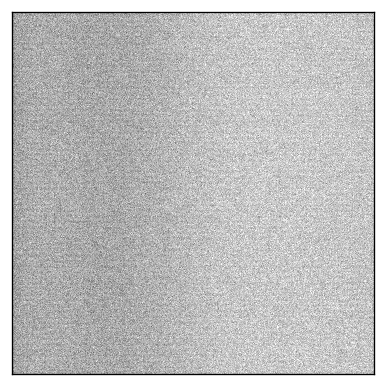
\includegraphics[scale=\myscale]{darkField_pst}
\end{tabular}
\caption{
The median of background (white and dark) images collected before and after the tomography scan.
The dynamic range of the white field images are $[0,4000]$ (counts) while the dynamic range of the dark field image is $[0,10]$ (counts).
}\label{fig: flat field images}
\end{figure}

Prior to the advanced background normalization, the analysis window is reduced from the detector size ($2048\times2048$) to the sample region ($500\times400$) such that the reduced image stack (\SI{\sim7}{GB}) can fit in a modern computer with double precision (64bit float).
Given that impulse noise is a common issue in high-energy tomography characterization, selective median filter
\footnote{
The selective median filter replace the outliers (impulse noises) with the median value calculated within a given kernel.
} 
was applied to each individual sinogram to reduce the impulse noises (\cref{fig: noise reduction}).

% --- noise reduction
\renewcommand{\myscale}{1}
\begin{figure}[htp]
\centering
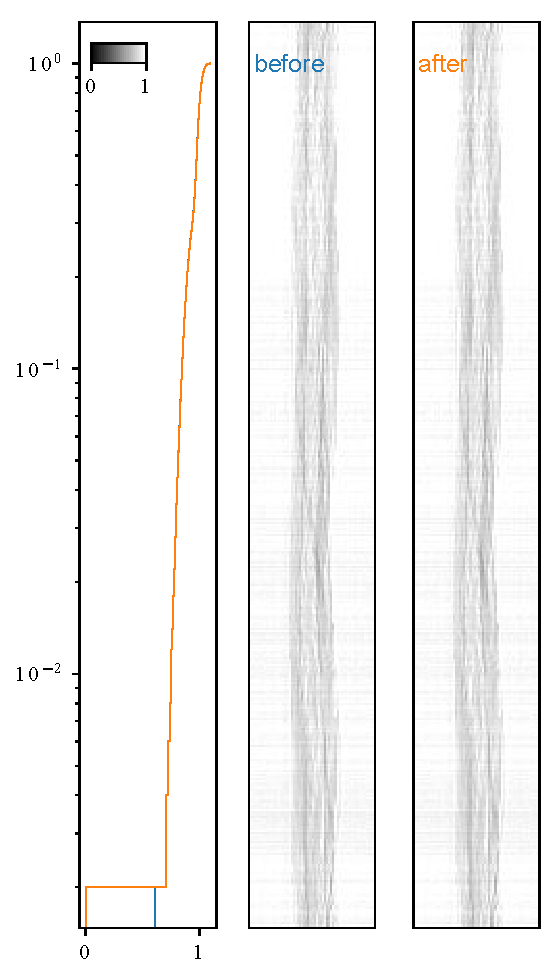
\includegraphics[scale=\myscale]{sinogramDenoise_retouched}
\caption{
Remove impulse noise from one example sinogram using selective median filter with a $3\times3$ kernel.
}\label{fig: noise reduction}
\end{figure}

For a normalized sinogram from an ideal tomography characterization, the dark region of the sinogram ($<1$) denotes the sample attenuation strength whereas the rest (air) should be white ($=1$).
However, the residual beam characteristics due to beam wiggling and intensity fluctuation often leaves horizontal linear features observed in \cref{fig: noise reduction}, which can be removed by rescaling each row of the sinogram such that the air region remains one (zero attenuation).
In this study, this process is automated with the following algorithm
%
\begin{itemize}
\item Calculate the cumulative intensity profile of each sinogram $i$ using $I_i = \sum_\omega I^\omega_i$.
\item Use the second order derivative of $I_i$ to locate the left and right air stripes for each sinogram $i$.
\item For each sinogram $i$, calculate the average intensity for each row in the left and right air stripes.
\item For each sinogram $i$, rescale the intensity of each row such that the average intensity in the left and right air stripes are one.
\item Calculate the total intensity difference $\Delta I$ due to the advanced normalization.
\item Repeat previous steps until $\Delta I$ falls below certain tolerance.
\end{itemize}

In this study, it was found that a total number of ten iterations
\footnote{
One might also argue that one iteration is sufficient as $\Delta I$ decays rapidly as shown in the left most figures of \cref{fig: sino norm top,fig: sino norm mid,fig: sino norm bot}
} of the advanced background normalization can successfully remove the horizontal linear artifacts in each sinogram, regardless of the signal to noise ratios (\cref{fig: sino norm top,fig: sino norm mid,fig: sino norm bot}).
Furthermore, it was found that that beam has minimum wiggling during this HETXM experiment as no obvious gradient can be found in each row of the difference sinogram (the right most sinograms in \cref{fig: sino norm top,fig: sino norm mid,fig: sino norm bot}).

% --- bg lvl norm
\renewcommand{\myscale}{0.5}
\begin{figure}
\centering
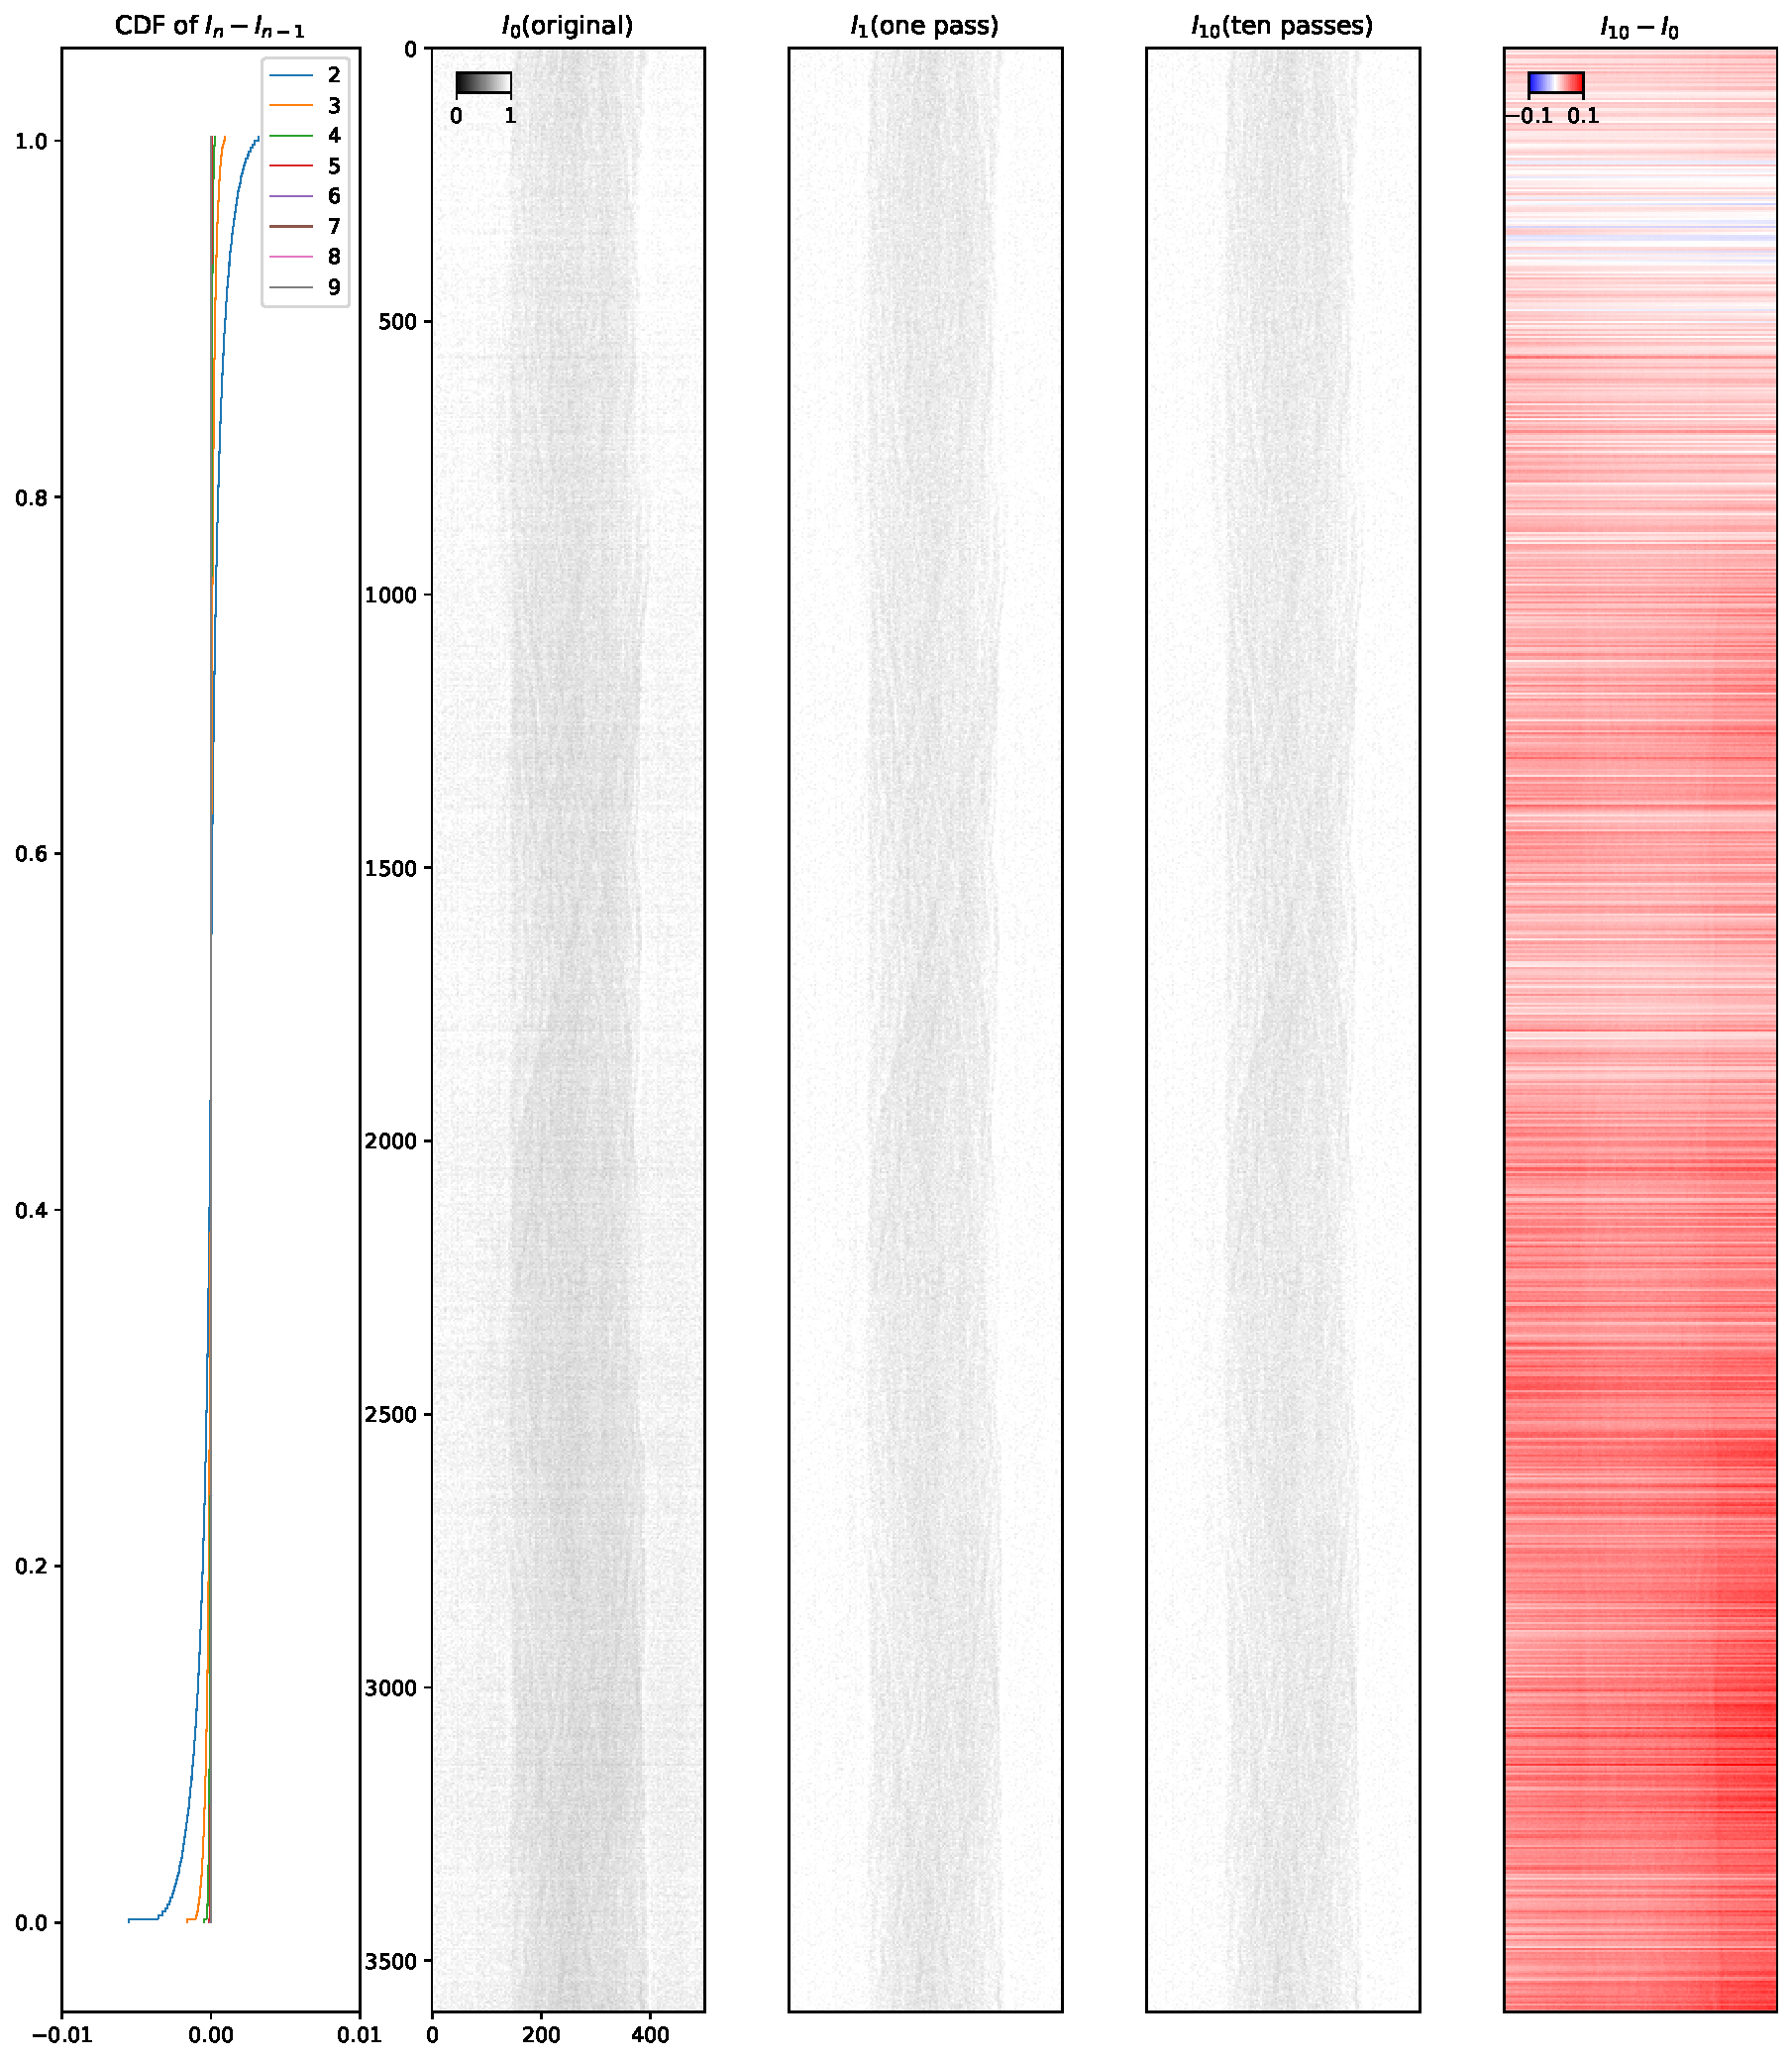
\includegraphics[scale=\myscale]{sinogramNormalization_top}
\caption{
Demonstration of the advanced background normalization in the top region of the projections with relatively \textbf{low} signal to noise ratio.
}\label{fig: sino norm top}
\end{figure}

\begin{figure}
\centering
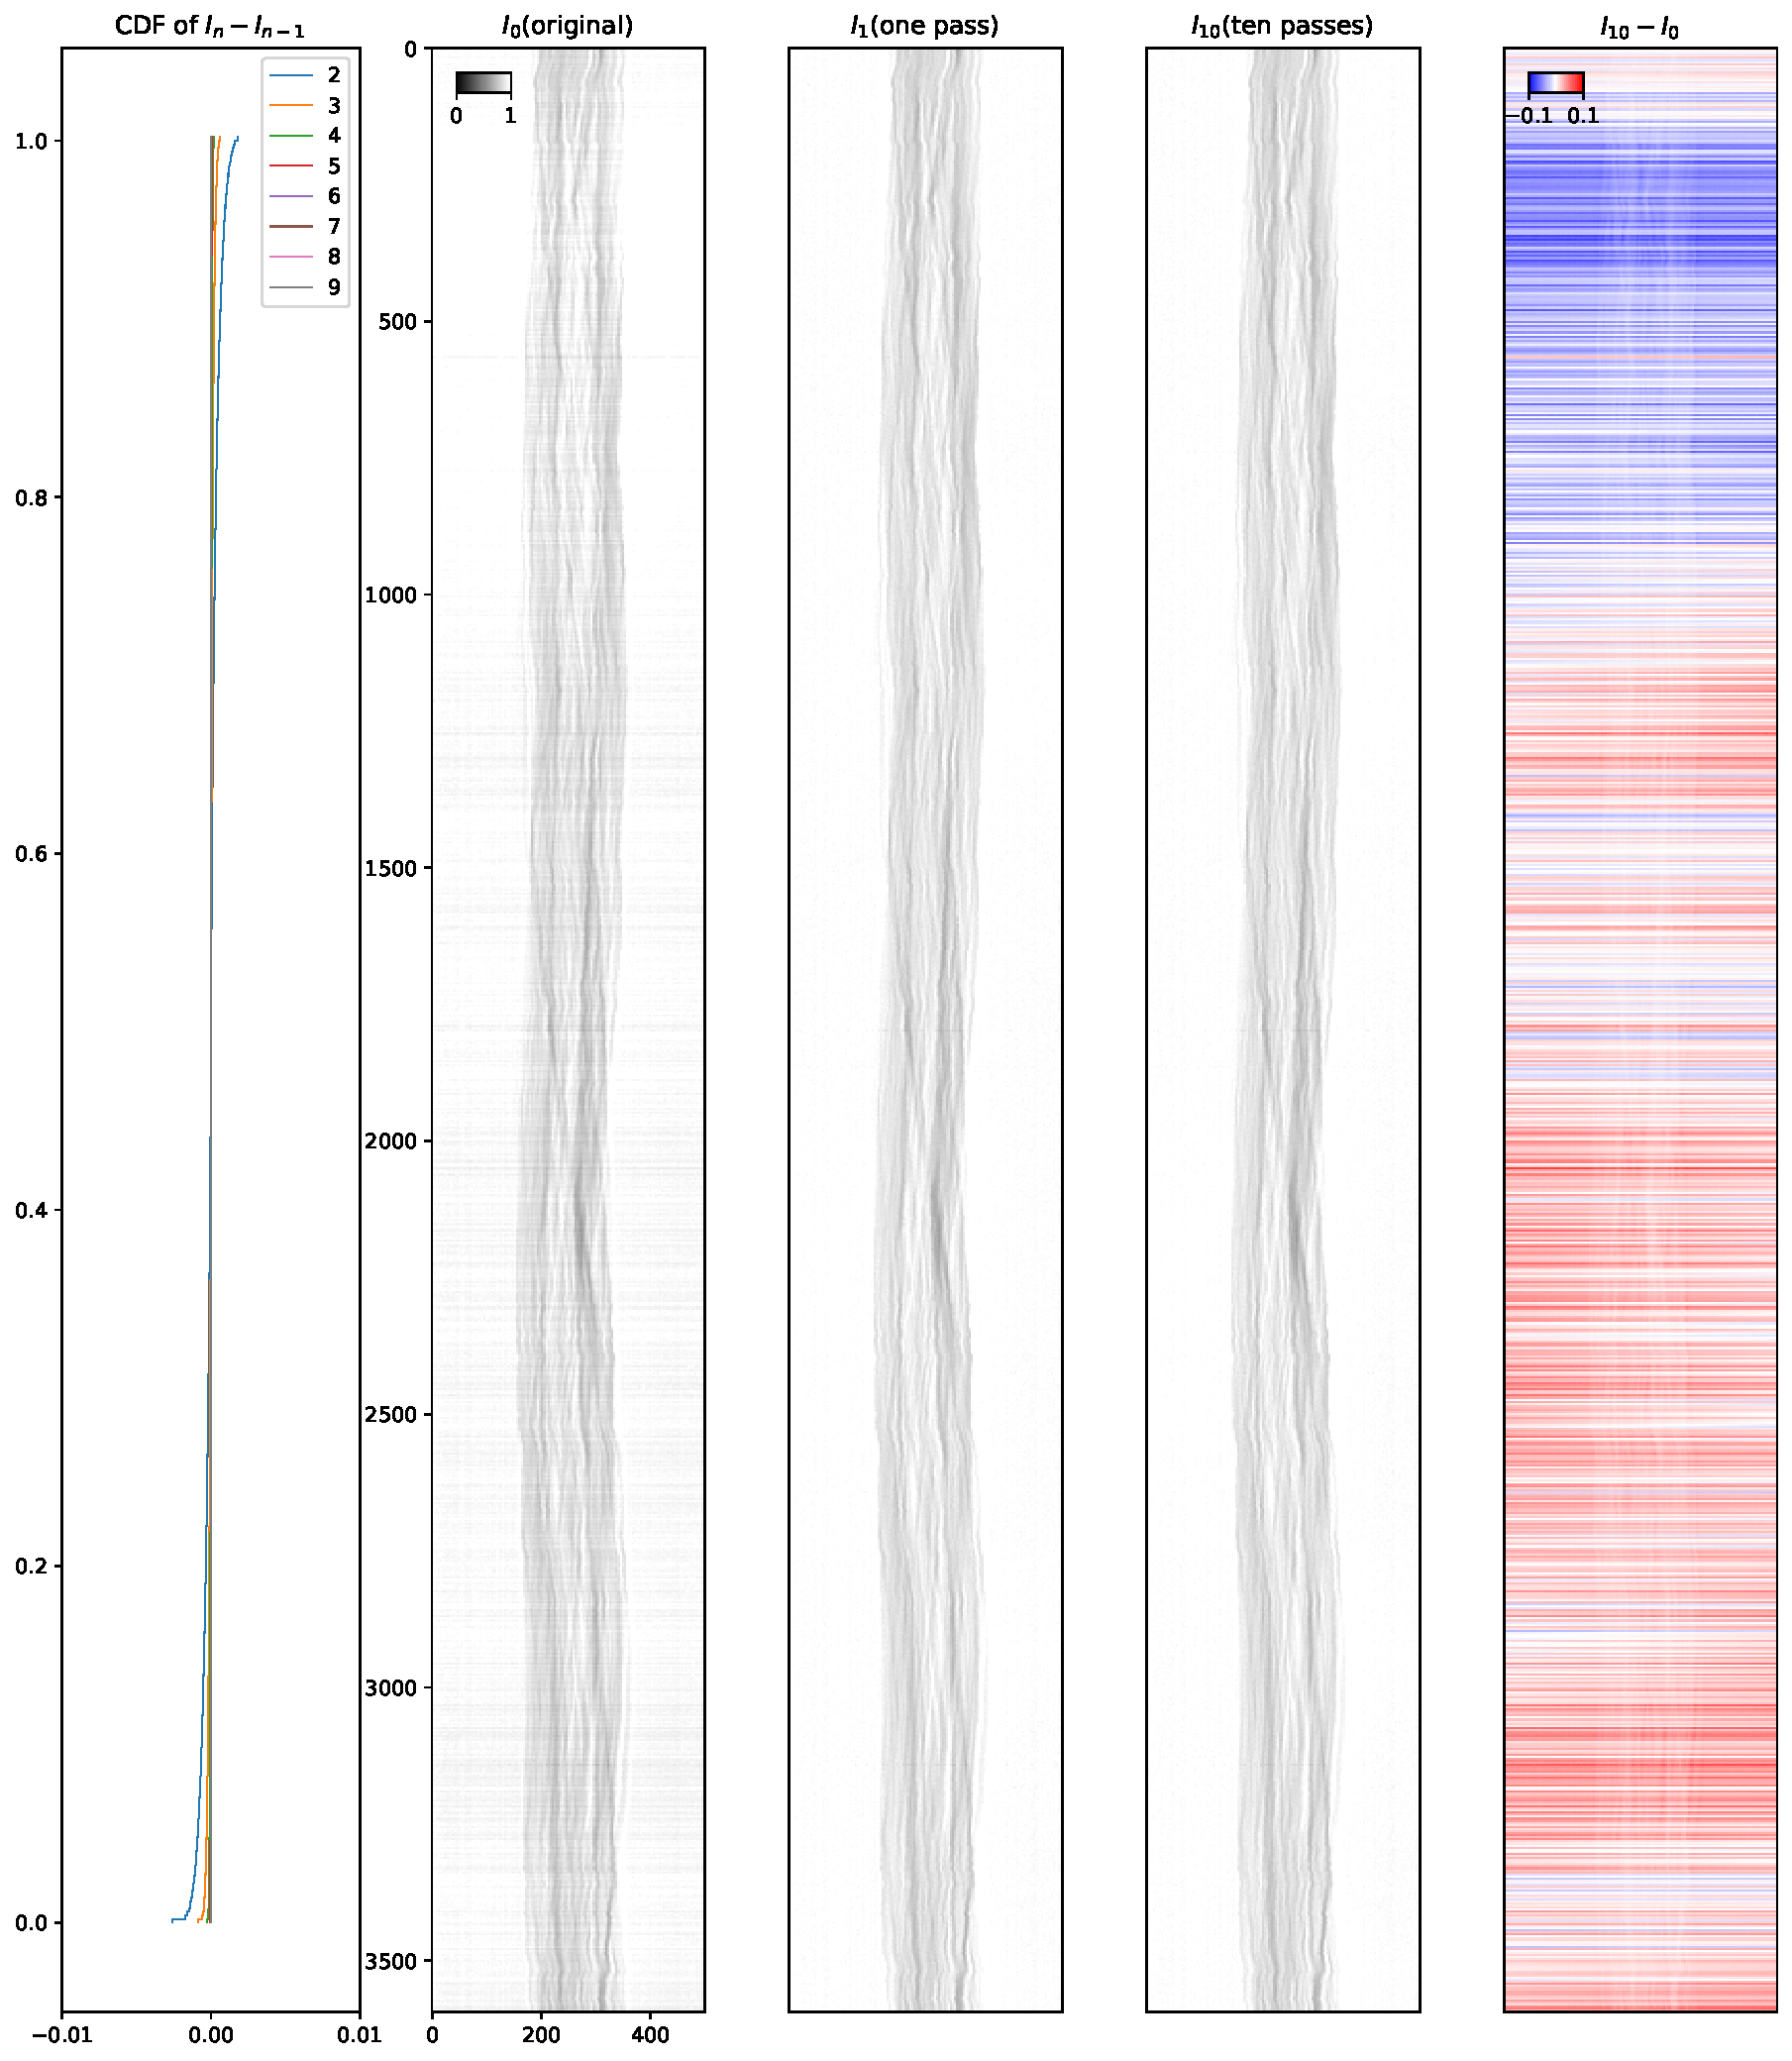
\includegraphics[scale=\myscale]{sinogramNormalization_middle}
\caption{
Demonstration of the advanced background normalization in the middle region of the sample with relatively \textbf{high} signal to noise ratio.
}\label{fig: sino norm mid}
\end{figure}

\begin{figure}
\centering
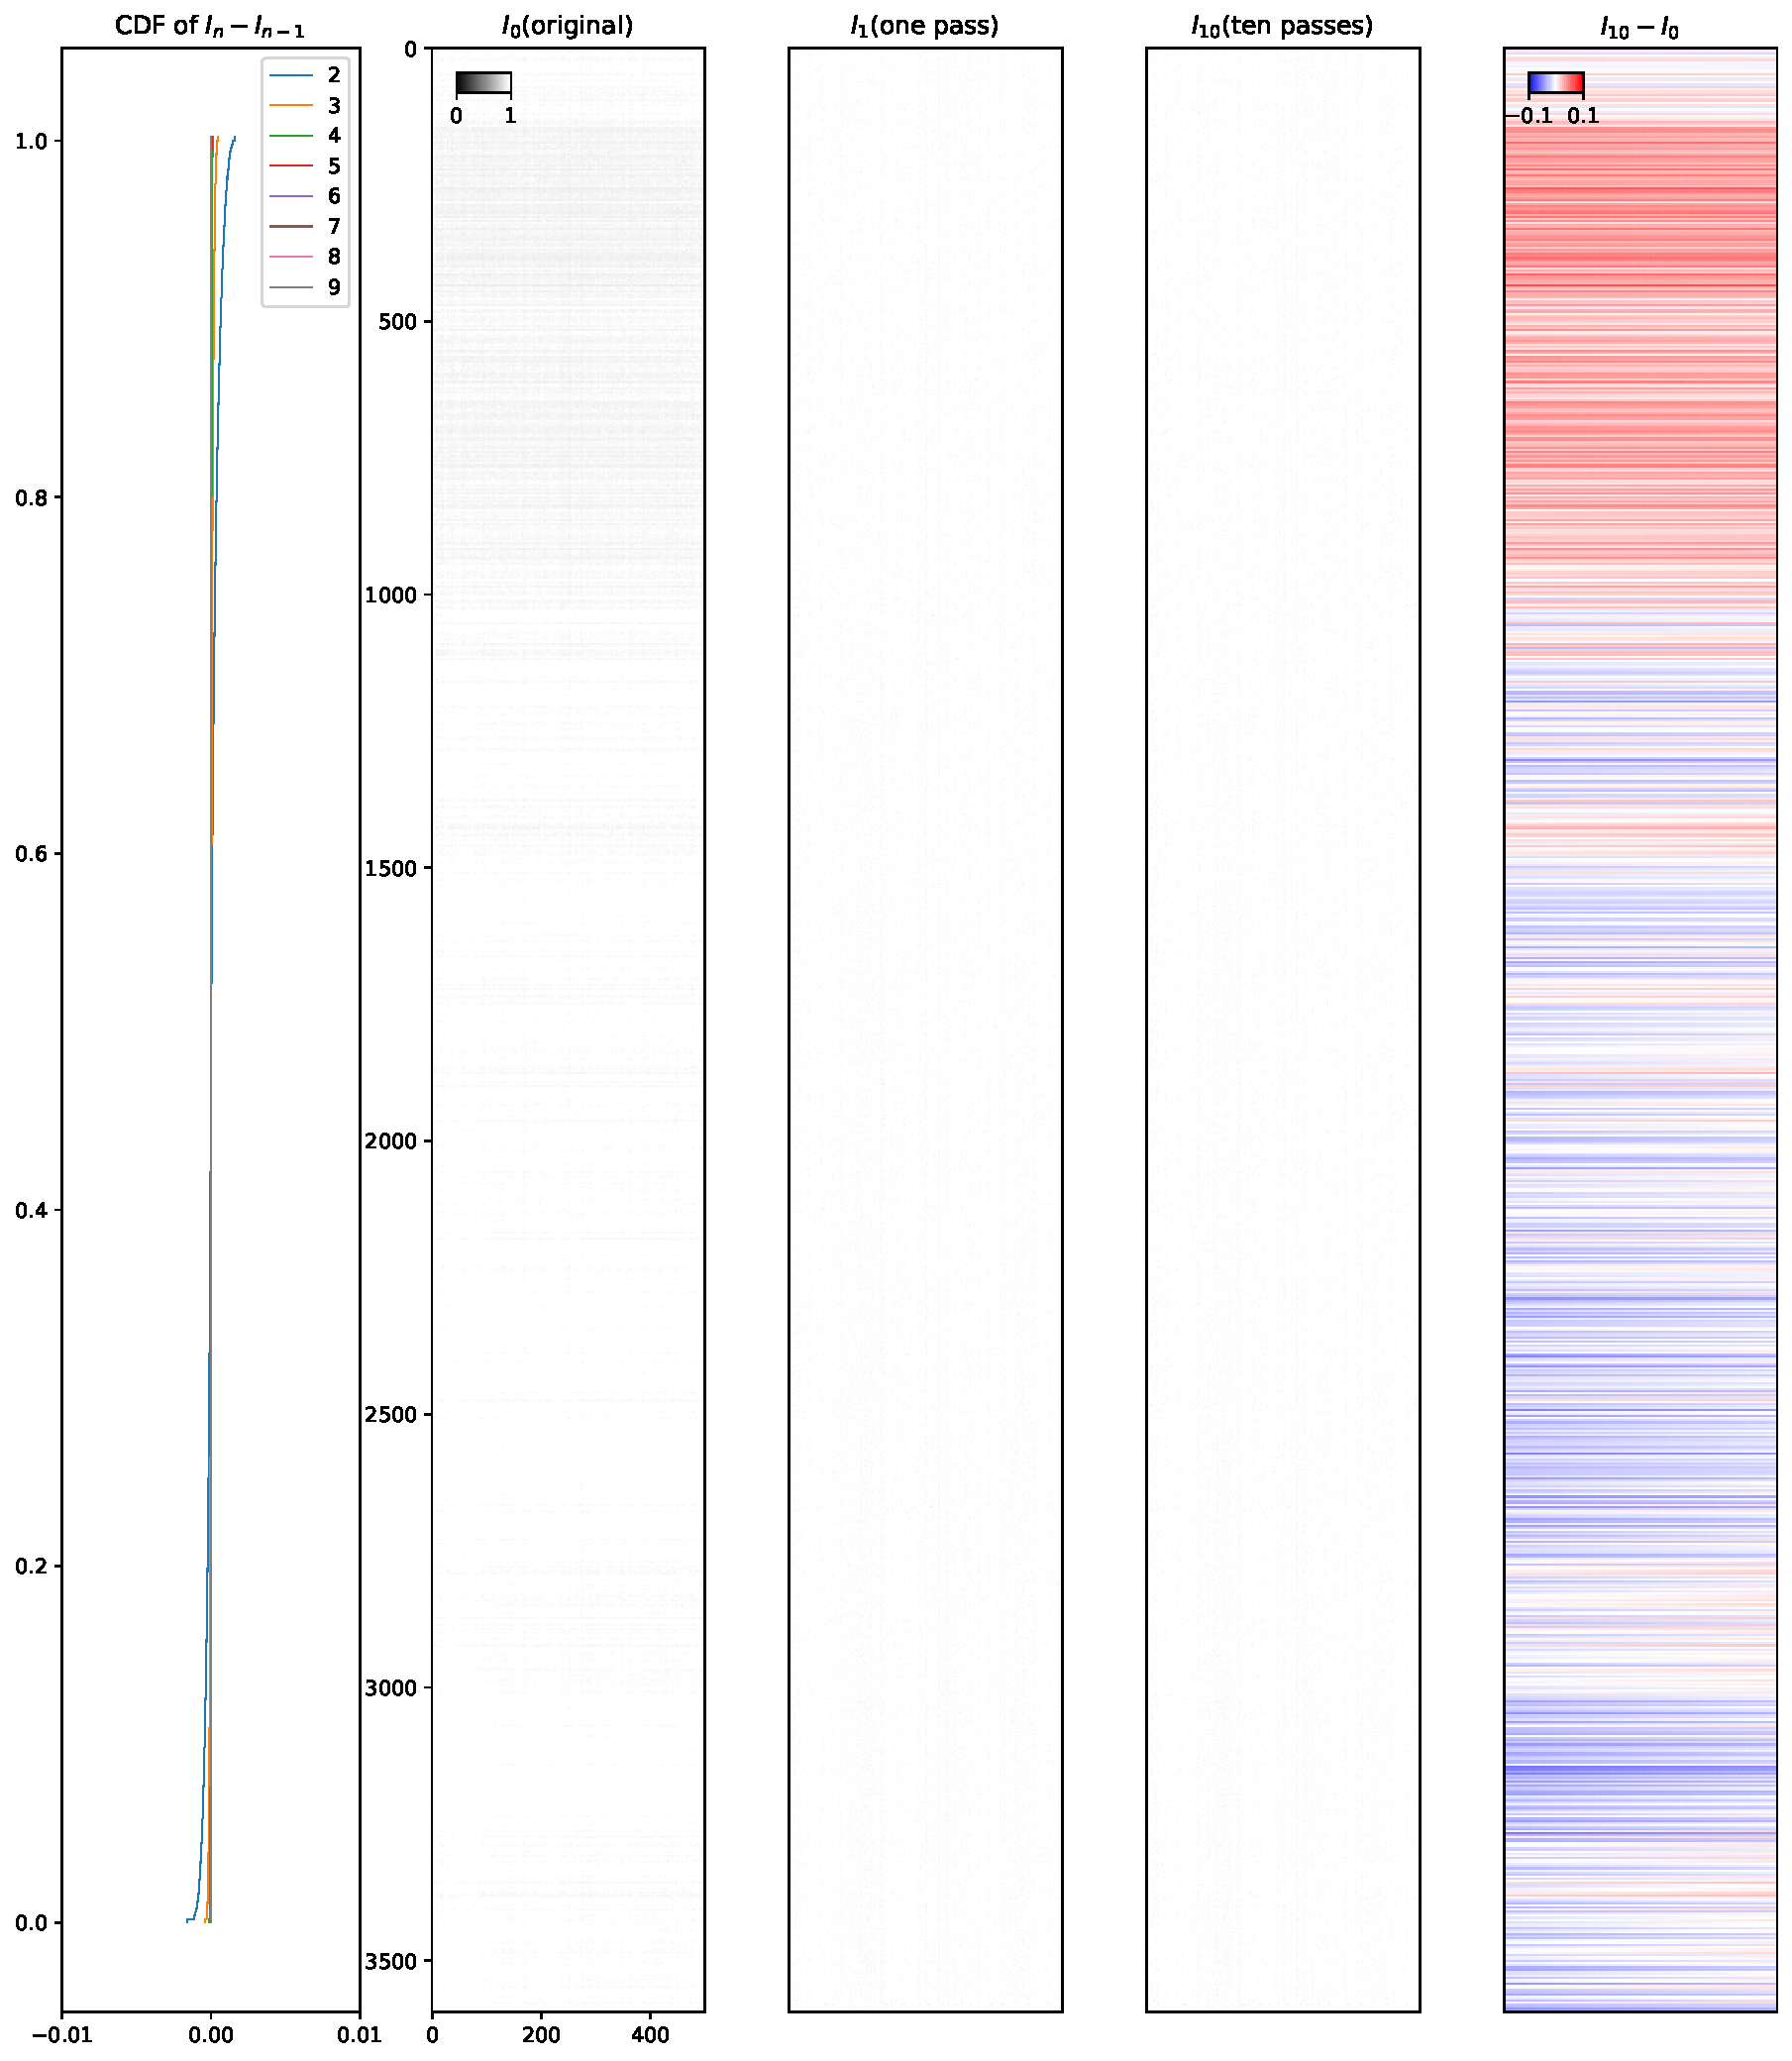
\includegraphics[scale=\myscale]{sinogramNormalization_bottom}
\caption{
Demonstration of the advanced background normalization in the bottom region of the projections with \textbf{no} sample signals.
}\label{fig: sino norm bot}
\end{figure}


\subsubsection{
Correction for dynamic misalignment
}\label{sec: correct dynamic misalignment}

In an ideal tomography characterization setting, a single rotation axis is shared by all \ang{180}-pair of projections due to the nature of the experiment.
However, dynamic misalignment could occur during the experiment due to the shifting/drifting/vibration of both the detector and sample stage.
For conventional high-energy tomography characterization, this effect is often well-below the experiment resolution, rendering its negative impact negligible.
This unfortunately does not hold true for HETXM due to its innate high spatial resolution, which often results in the appeared sample jittering in the collected projections.

Using the center column of the projection image as a reference, one could correct the horizontal component of the dynamic misalignment by systematically shifting the rotation axis of \ang{180}-pair projections to the reference rotation axis.
In this study, this process was realized as the following steps:
%
\begin{itemize}
\item 
Calculate the pair-wise rotation center (horizontal component of the rotation axis) of each \ang{180}-pair using a sub-pixel image registration algorithm developed by \citet{Guizar-Sicairos_etal2008}.
\item 
Calculate the difference ($\delta_h$) between the pair-wise rotation center and the horizontal center of the projection image (\cref{fig: corrupted frame detection}).
\item 
Inspect the pairs with extremely large deviation (outliers), and remove the pairs contain corrupted frames (\cref{fig: corrupted frames}).
\item
Shift each \ang{180}-pair of projections such that all projection images share the same rotation axis (the reference rotation axis).
\end{itemize}

% --- corrupted frame detection
\renewcommand{\myscale}{1}
\begin{figure}[htp]
\centering
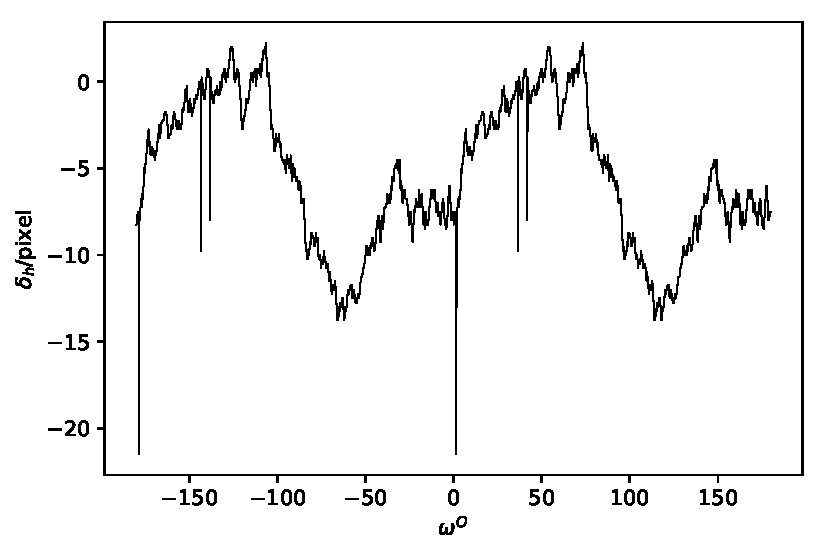
\includegraphics[scale=\myscale]{corruptedFrameDetection}
\caption{
The corrupted frames can be detected by checking the outliers in the profile of \ang{180} pair-wise rotation axis where $\delta_h$ denotes the amount of horizontal offset between rotation axis and the image center column.
}\label{fig: corrupted frame detection}
\end{figure} 

% --- detected corrupted frames
\renewcommand{\myscale}{0.5}
\begin{figure}[htp]
\centering
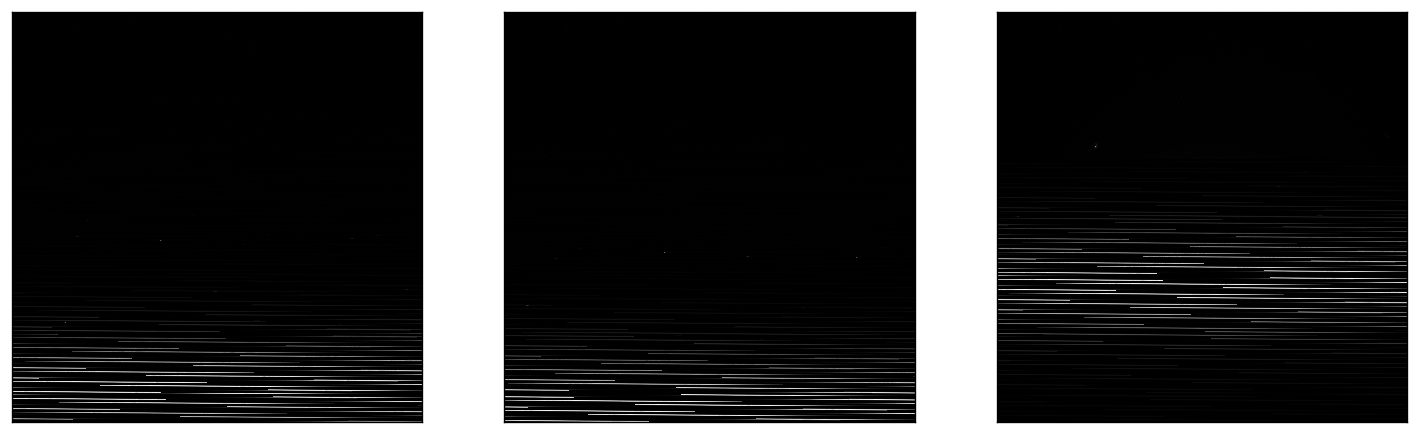
\includegraphics[scale=\myscale]{corruptedFrames}
\caption{
Three corrupted frames were detected out of the total 3600 frames.
These corrupted frames and the associated \ang{180} pairs were excluded from the tomography reconstruction as it is not possible to adjust a \ang{180} pair horizontally with one corrupted frame.
}\label{fig: corrupted frames}
\end{figure}

In theory, one should also correct for the \textbf{vertical} component of the dynamic misalignment.
However, this was deemed impossible with current HETXM configuration due to \textit{the lack of a common reference point}.
Therefore, the vertical component of the dynamic misalignment was left uncorrected in this study.


\subsection{Tomography reconstruction}\label{sec: tomo recon}

Prior to the actual tomography reconstruction,  a per slab based rotation axis deviation analysis was perform for the HETXM data set since a tilted rotation axis is a common problem in standard tomography characterization.
More specifically, four \ang{180}-pair of projections were randomly selected from the tomography projection image stacks.
Each pair is then vertically divided into 200 slabs with thickness of two pixels.
The same image registration based method was used to calculate the rotation axis for each slab in each pair.
These per slab based rotation axis centers were then used to calculate the relative deviation ($\delta_h$) with respect to the common reference rotation axis.
The general trend of the profile in \cref{fig: rotation axis tilt profile} ($\delta_h$ going from positive to negative when moving from top slabs to lower slabs) indicate that the rotation axis of this HETXM data set is indeed tilted.
Therefore, a per slab based tomography reconstruction was performed using the ``gridrec'' engine and ``hann'' filter from TomoPy \citep{Gursoy_etal2014}.
The resulting reconstruction results can be found in \cref{fig: recon demo}. 

% --- rotation axis tilt
\renewcommand{\myscale}{1.0}
\begin{figure}[htp]
\centering
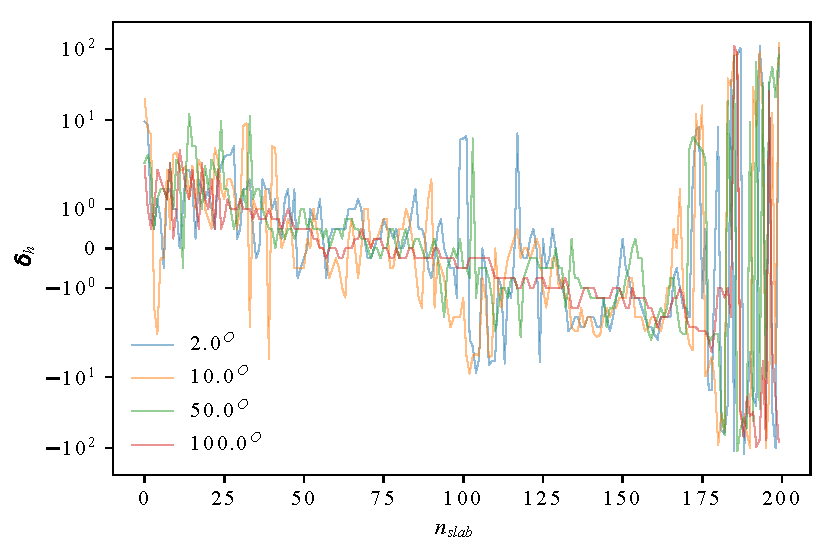
\includegraphics[scale=\myscale]{rotationAxisTiltDemo_retouched}
\caption{
The per slab (2 pixels) based rotation axis deviation profile of four \ang{180}-pair projections indicates that the rotation axis of the collected tomography projection image stack is tilted, which results in the consistent trend going from positive (top) to negative (bottom).
}\label{fig: rotation axis tilt profile}
\end{figure}

% --- reconstruction results
\renewcommand{\myscale}{0.3}
\begin{figure}[htp]
\centering
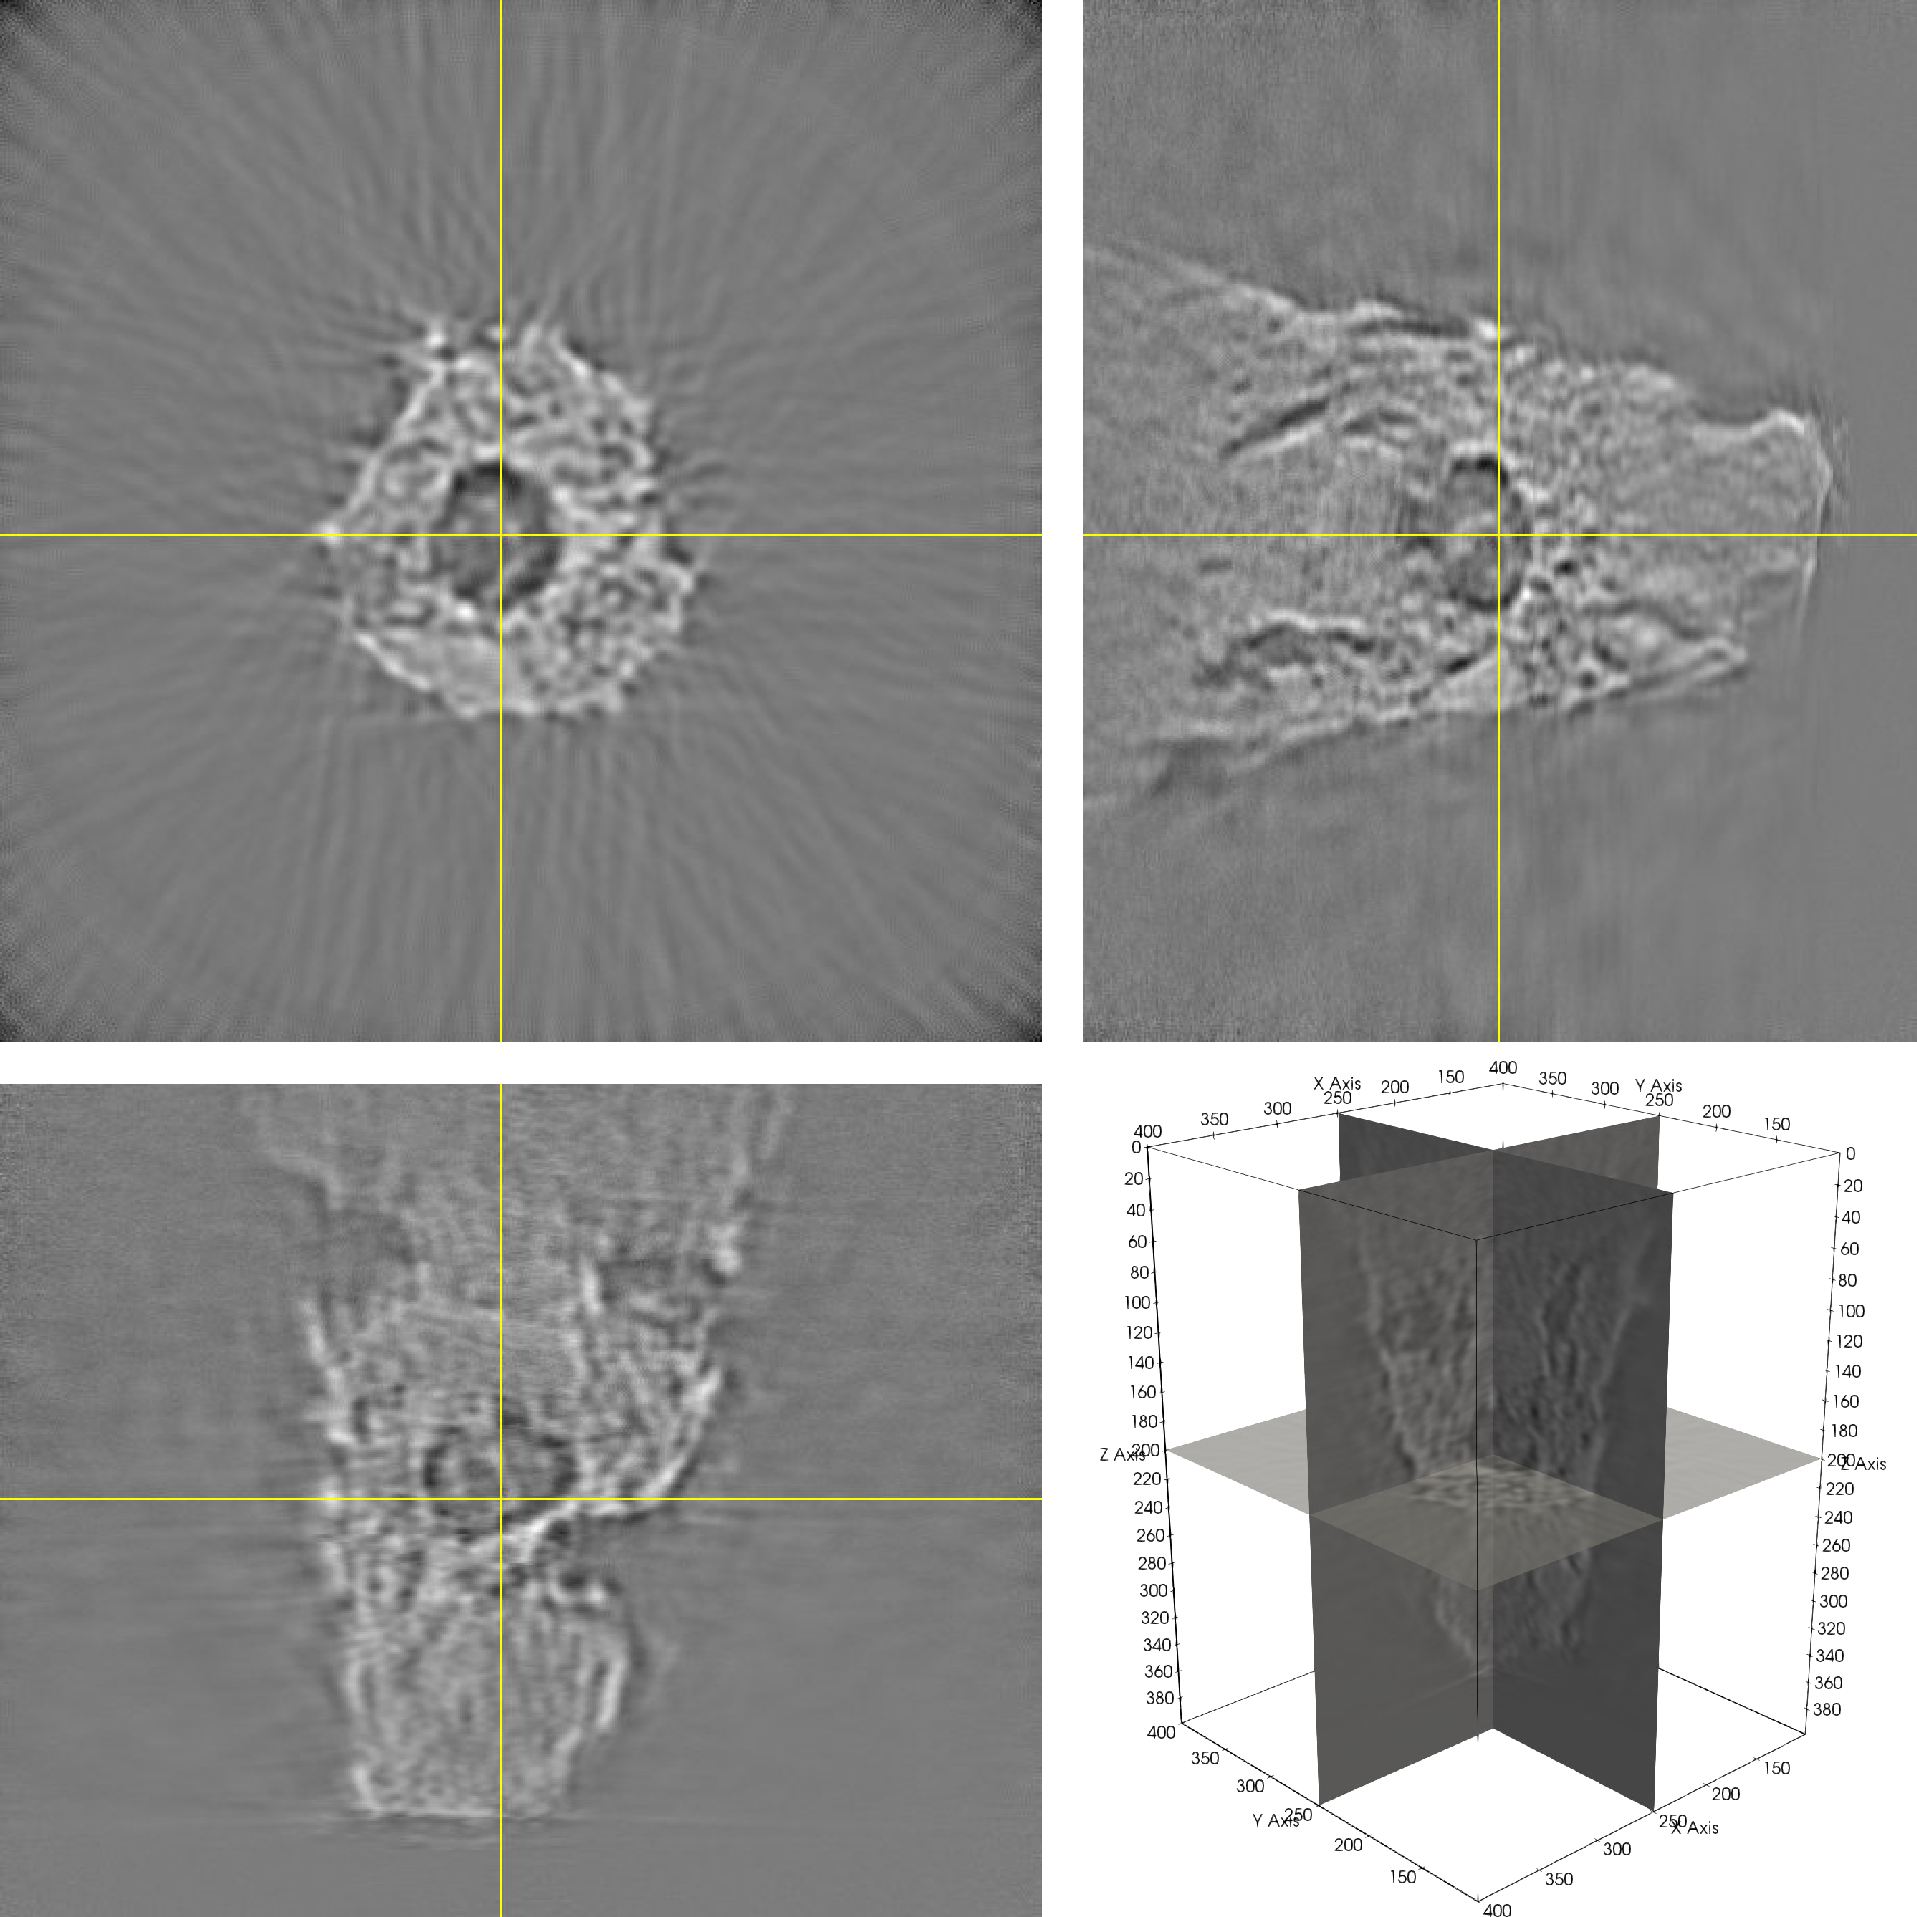
\includegraphics[scale=\myscale]{recon_demo}
\caption{
Orthogonal slices of the tomography reconstruction results show evident porous characteristics of the tip of the SOFC. 
}\label{fig: recon demo}
\end{figure}


% ----- Void characterization ----- %
\section{Porosity characterization}\label{sec: porosity characterization}

The tomography reconstruction results (\cref{fig: recon demo}) demonstrate evident porous characteristics of the tip of the SOFC.
In this section, the 2D porosity of the tip of SOFC is systematically characterized using phase retrieval in conjunction with \href{https://en.wikipedia.org/wiki/Blob_detection}{Laplacian of Gaussian (LOG)} based blob detection.

Despite the advanced background normalization performed in \cref{sec: bg norm}, there are still many relatively weak linear artifacts surrounding the reconstructed volume.
These linear features are commonly referred to as phase contrast artifacts, which can interfere with LOG based blob detection.
Therefore, a single image based phase retrieval method developed by \citet{Paganin_etal2002} was used to extract absorption and phase contrast maps from reconstruction results (\cref{fig: phase retrieval demo}).
The absorption maps provide a generate guide to locate the sample when used in conjunction with a circular mask that isolate the sample neighborhood.
Furthermore, it can also serve as a mask to suppress the unwanted linear phase contrast artifacts in the phase contrast map, resulting in a composite image that are more suitable for LOG-based blob detection.
An example of this 2D void characterization process is demonstrated in \cref{fig: void detection demo}.

% --- phase retrieve demonstration
\renewcommand{\myscale}{0.42}
\begin{figure}[htp]
\centering
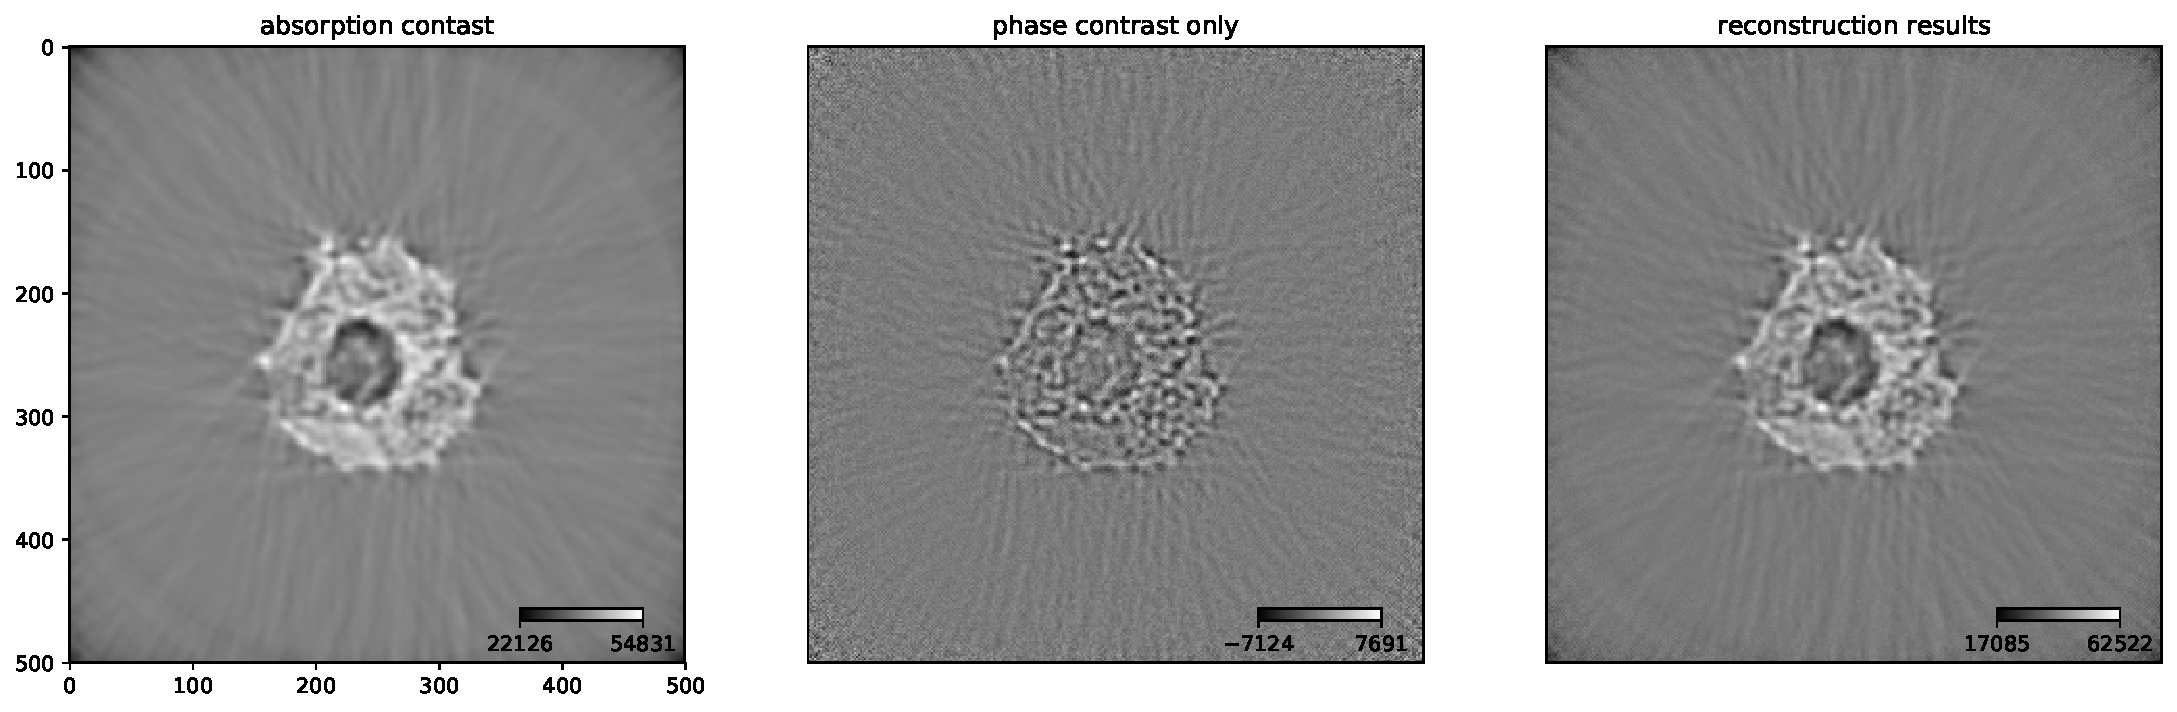
\includegraphics[scale=\myscale]{phaseRetrievalDemo}
\caption{
The absorption contrast (left) and the phase contrast (middle) are separated from the reconstruction results (right) using the method originally developed by \citet{Paganin_etal2002}.
}\label{fig: phase retrieval demo}
\end{figure}

% --- void detection demo
\renewcommand{\myscale}{.5}
\begin{figure}
\centering
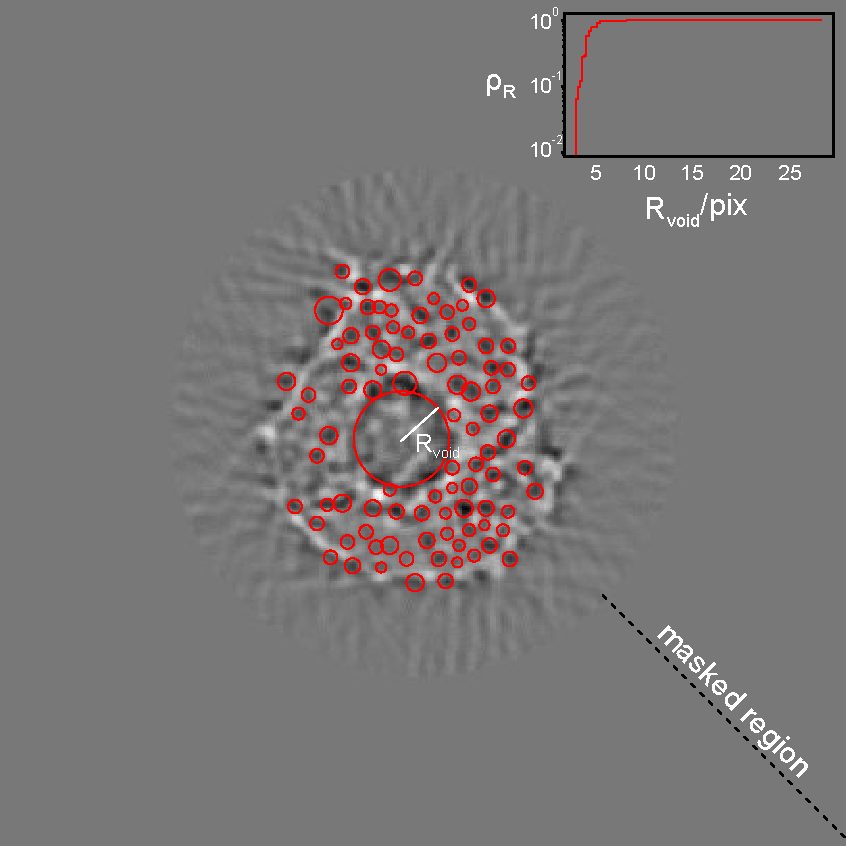
\includegraphics[scale=\myscale]{voidDetectionDemo_mid}
\caption{
LOG-based blob detection was used to identify the void features (highlighted with \textcolor{red}{O}) in a 2D slice of the reconstruction results.
The cumulative distribution function of the 2D void radius ($R_\text{void}$) is super imposed at the upper right corner of the image.
A circular mask is used to isolate the sample, which improves the efficiency of the porosity characterization by limiting the analysis scope to the sample neighborhood only.
}\label{fig: void detection demo}
\end{figure}

The 2D void characterization process was performed for all 400 slices of the reconstruction results, the results of which are shown as a 2D histogram of the 2D void counts with respect to the slice position and void size (\cref{fig: void profile}).
According to this 2D histogram, the majority of the voids are present near the base of the tip, mostly with a radius of \SI{1}{\micro\meter}.
As moving towards the middle section of the tip, some large voids (\SI{15}{\micro\meter}) started to appear, while the total number of voids continue to decline.
While moving from the middle section to the tip at the bottom, the number of both large and small voids decreases rapidly, leading to about 1 void per \SI{0.4}{\square\micro\meter} near the very end.
 
% --- porosity profile
\renewcommand{\myscale}{1.0}
\begin{figure}[htp]
\centering
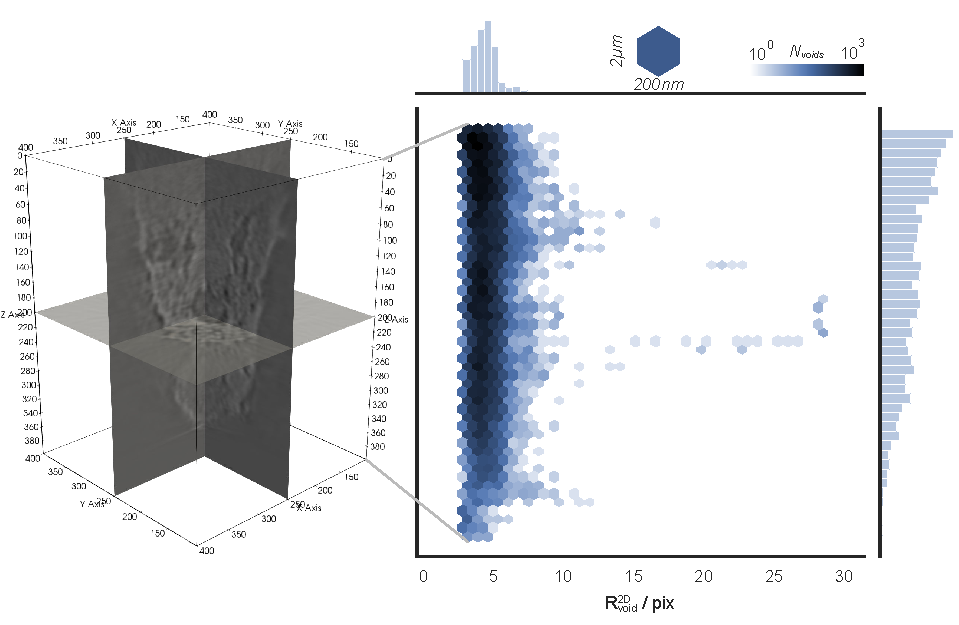
\includegraphics[scale=\myscale]{void_profile}
\caption{
The 2D histogram of the 2D void counts with respect to the slice position and the void radius (2D), along with the associated 1D distribution along the axis of slice position (right) and void size (top). 
The count in each bin is plotted on a log color scale.
}\label{fig: void profile}
\end{figure}


% ----- summary ----- %
\section{Summary}\label{sec: summary}

In this study, the porous structure of the tip of a SOFC cathode is characterized using HETXM.
After correction for beam instability and dynamic misalignment, the associated 

% ----- reference ----- %
\bibliographystyle{plainnat}
\bibliography{tmxSOFC_tomoReport}

\end{document}
